%% LyX 2.3.6 created this file.  For more info, see http://www.lyx.org/.
%% Do not edit unless you really know what you are doing.
\documentclass[10pt]{article}
\usepackage{helvet}
\renewcommand{\familydefault}{\sfdefault}
\usepackage[T1]{fontenc}
\usepackage[latin9]{inputenc}
\usepackage[a4paper]{geometry}
\geometry{verbose,tmargin=2cm,bmargin=4cm,lmargin=2cm,rmargin=2cm}
\usepackage{fancyhdr}
\pagestyle{fancy}
\setlength{\parskip}{6pt}
\setlength{\parindent}{0pt}
\usepackage{tcolorbox}
\usepackage{amsmath}
\usepackage{amsthm}
\usepackage{amssymb}
\usepackage{graphicx}

\makeatletter

%%%%%%%%%%%%%%%%%%%%%%%%%%%%%% LyX specific LaTeX commands.
%% A simple dot to overcome graphicx limitations
\newcommand{\lyxdot}{.}


%%%%%%%%%%%%%%%%%%%%%%%%%%%%%% User specified LaTeX commands.
\usepackage{tcolorbox}
\usepackage{amsthm}
\usepackage{lastpage}
\usepackage{fancyhdr}
\usepackage{accents}
\usepackage{titlesec}
\usepackage{marginnote}


\usepackage{enumitem}
\setlist{nolistsep}

\usepackage{tcolorbox}
\definecolor{light-blue}{cmyk}{0.24, 0.12, 0.0, 0.04, 1.00}


%

%parskip shold take care of heading spacing
\titlespacing\section{0pt}{0pt}{0pt}
\titlespacing\subsection{0pt}{0pt}{0pt}
\titlespacing\subsubsection{0pt}{0pt}{0pt}



\setlength{\headheight}{40pt}

\makeatother

\begin{document}
\lhead{Neimhin Robinson Gunning (16321701)} \rhead{CS7CS4 Week 8 Assignment} 

\begin{tcolorbox}[colback=light-blue]
\begin{small} \textbf{DECLARATION:} I understand that this is an
\textbf{individual} assessment and that collaboration is not permitted.
I have read, understand and agree to abide by the plagiarism provisions
in the General Regulations of the University Calendar for the current
year, found at http://www.tcd.ie/calendar. I understand that by returning
this declaration with my work, I am agreeing with the above statement.
\end{small} 
\end{tcolorbox}

\bigskip{}


\section{(i)}

The results of a 2D convolution function applied to a single-channel
image, with two different kernels, are presented in Figure \ref{fig:A-200x200-RGB}.

\begin{figure}
\begin{centering}

\includegraphics[width=0.25\textwidth]{fig/red_triangle200x200}~~~~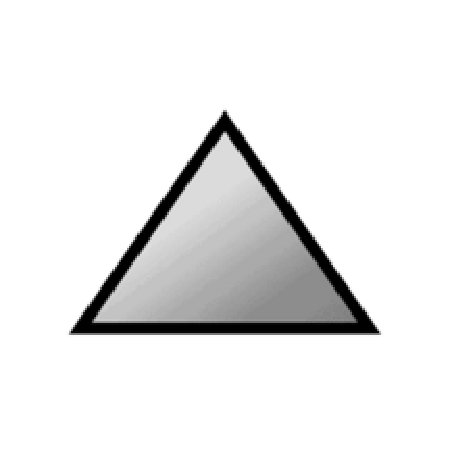
\includegraphics[width=0.25\textwidth]{fig/red_triangle-red-channel}
\par\end{centering}
\begin{centering}
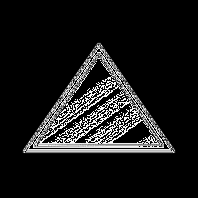
\includegraphics[width=0.25\textwidth]{fig/red_triangle-convolve-one}~~~~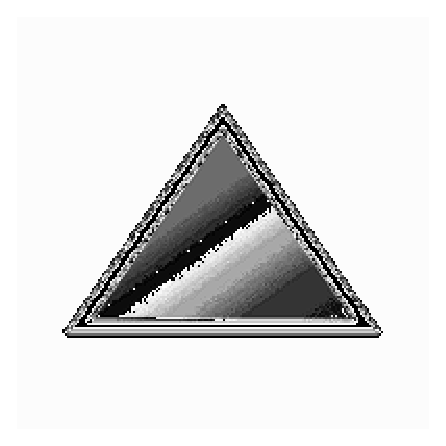
\includegraphics[width=0.25\textwidth]{fig/red_triangle-convolve-two}
\par\end{centering}
\begin{centering}
$k_{1}=\left[\begin{array}{ccc}
-1 & -1 & -1\\
-1 & 8 & -1\\
-1 & -1 & -1
\end{array}\right]$~~~~~~~~$k_{2}=\left[\begin{array}{ccc}
0 & -1 & 0\\
-1 & 8 & -1\\
0 & -1 & 0
\end{array}\right]$
\par\end{centering}
\caption{\label{fig:A-200x200-RGB}A 200x200 RGB image (top left) has green
and blue channels removed resulting in a grayscale image (top right).
The image is convolved with two kernels, $k_{1}$ (bottom left), and
$k_{1}$ (bottom right).}

\end{figure}


\section{(ii)}

\subsection{(ii) (a) model layers, kernels, channels}

In Figure \ref{fig:code} is the python source code for a CNN with 4 convolution layers.
The input to the model is a tensor with shape (32,32,3), i.e. an RGB
image with 32x32 pixels.

\begin{figure}
\includegraphics[width=1\textwidth]{fig/model_architecture\lyxdot py}
\caption{\label{fig:code}Source code of a ConvNet keras model.}
\end{figure}

The CNN layers of the model have the following structures:
\begin{enumerate}
\item (line 7): input=(32,32,3), number of kernels=16, kernel shape=(3,3,3),
output shape=(32,32,16)
\item (line 8): input=(32,32,16), number of kernels=16, kernel shape=(3,3,16),
output shape=(16,16,16)
\item (line 9): input shape=(16,16,16), number of kernels=32, kernel shape=(3,3,16),
output shape=(16,16,32)
\item (line 10): input shape=(16,16,32), number of kernels=32, kernel shape=(3,3,32),
output shape=(8,8,32)
\end{enumerate}
The next layer is a dropout layer which randomly sets on average 50\%
of its inputs to 0 and leaves the rest of the inputs the same. Its
input and output shape is (8,8,32). The next layer simply unravels
the (8,8,32) tensor into an array of length $2048=8\cdot8\cdot32$.
The final layer consists of 10 separate linear combinations of the previous layers outputs.
The output of this `Dense' layer is just the `softmax' function applied to the vector of ten linear combinations, $[ z_1, \ldots, z_{10}]$.

\begin{equation}
    \text{softmax}(z_i) = \frac{e^{z_i}}{\sum_{j=1}^{10} e^{z_j}}
\end{equation}

\begin{equation}
    \text{output of dense layer} = [ \text{softmax}(z_0), \text{softmax}(z_1), \ldots, \text{softmax}(z_{10}) ] 
\end{equation}


\subsection{(ii) (b) (i)}
Keras reports that model given by the code in Figure \ref{fig:code} has 37146 total parameters, all of which a trainable.
The final Dense layer has the most parameters, namely $2048\cdot10+10=20490$.
The number of parameters in a convolution layer is determined by the kernel size and the number of filters and the number of channels,
$\text{no. params}=k_w\cdot k_h\cdot c\cdot f$,
whereas the number of paramaters in a Dense layer is determined by the input and output sizes.
Since the input dimension for the Dense layer is quite large (2048), this layer ends up having more
parameters than any of the convolution layers.

The models evaluation scores are significantly better on the training data than they are on the test data.
On the training data the model has an accuracy of 57\%, and on the the test data is 48\%. The average $F_1$-score is 0.48.
A simple baseline which always predicts the most frequent class achieves an accuracy of 10\%, naturally considering the test set is balanced and there are ten classes,
and the average $F_1$-score across the classes in 0.018. The ConvNet is much better than the `most_frequent' baseline.

\subsection{(ii) (b) (ii)}
The history of loss and accuracy of the model trained on 5K samples over 20 epochs is presented in Figure \ref{fig:iibii-acc-loss}.
Generally improvements to loss and accuracy after each epoch are diminishing.

\begin{figure}
    \begin{centering}
        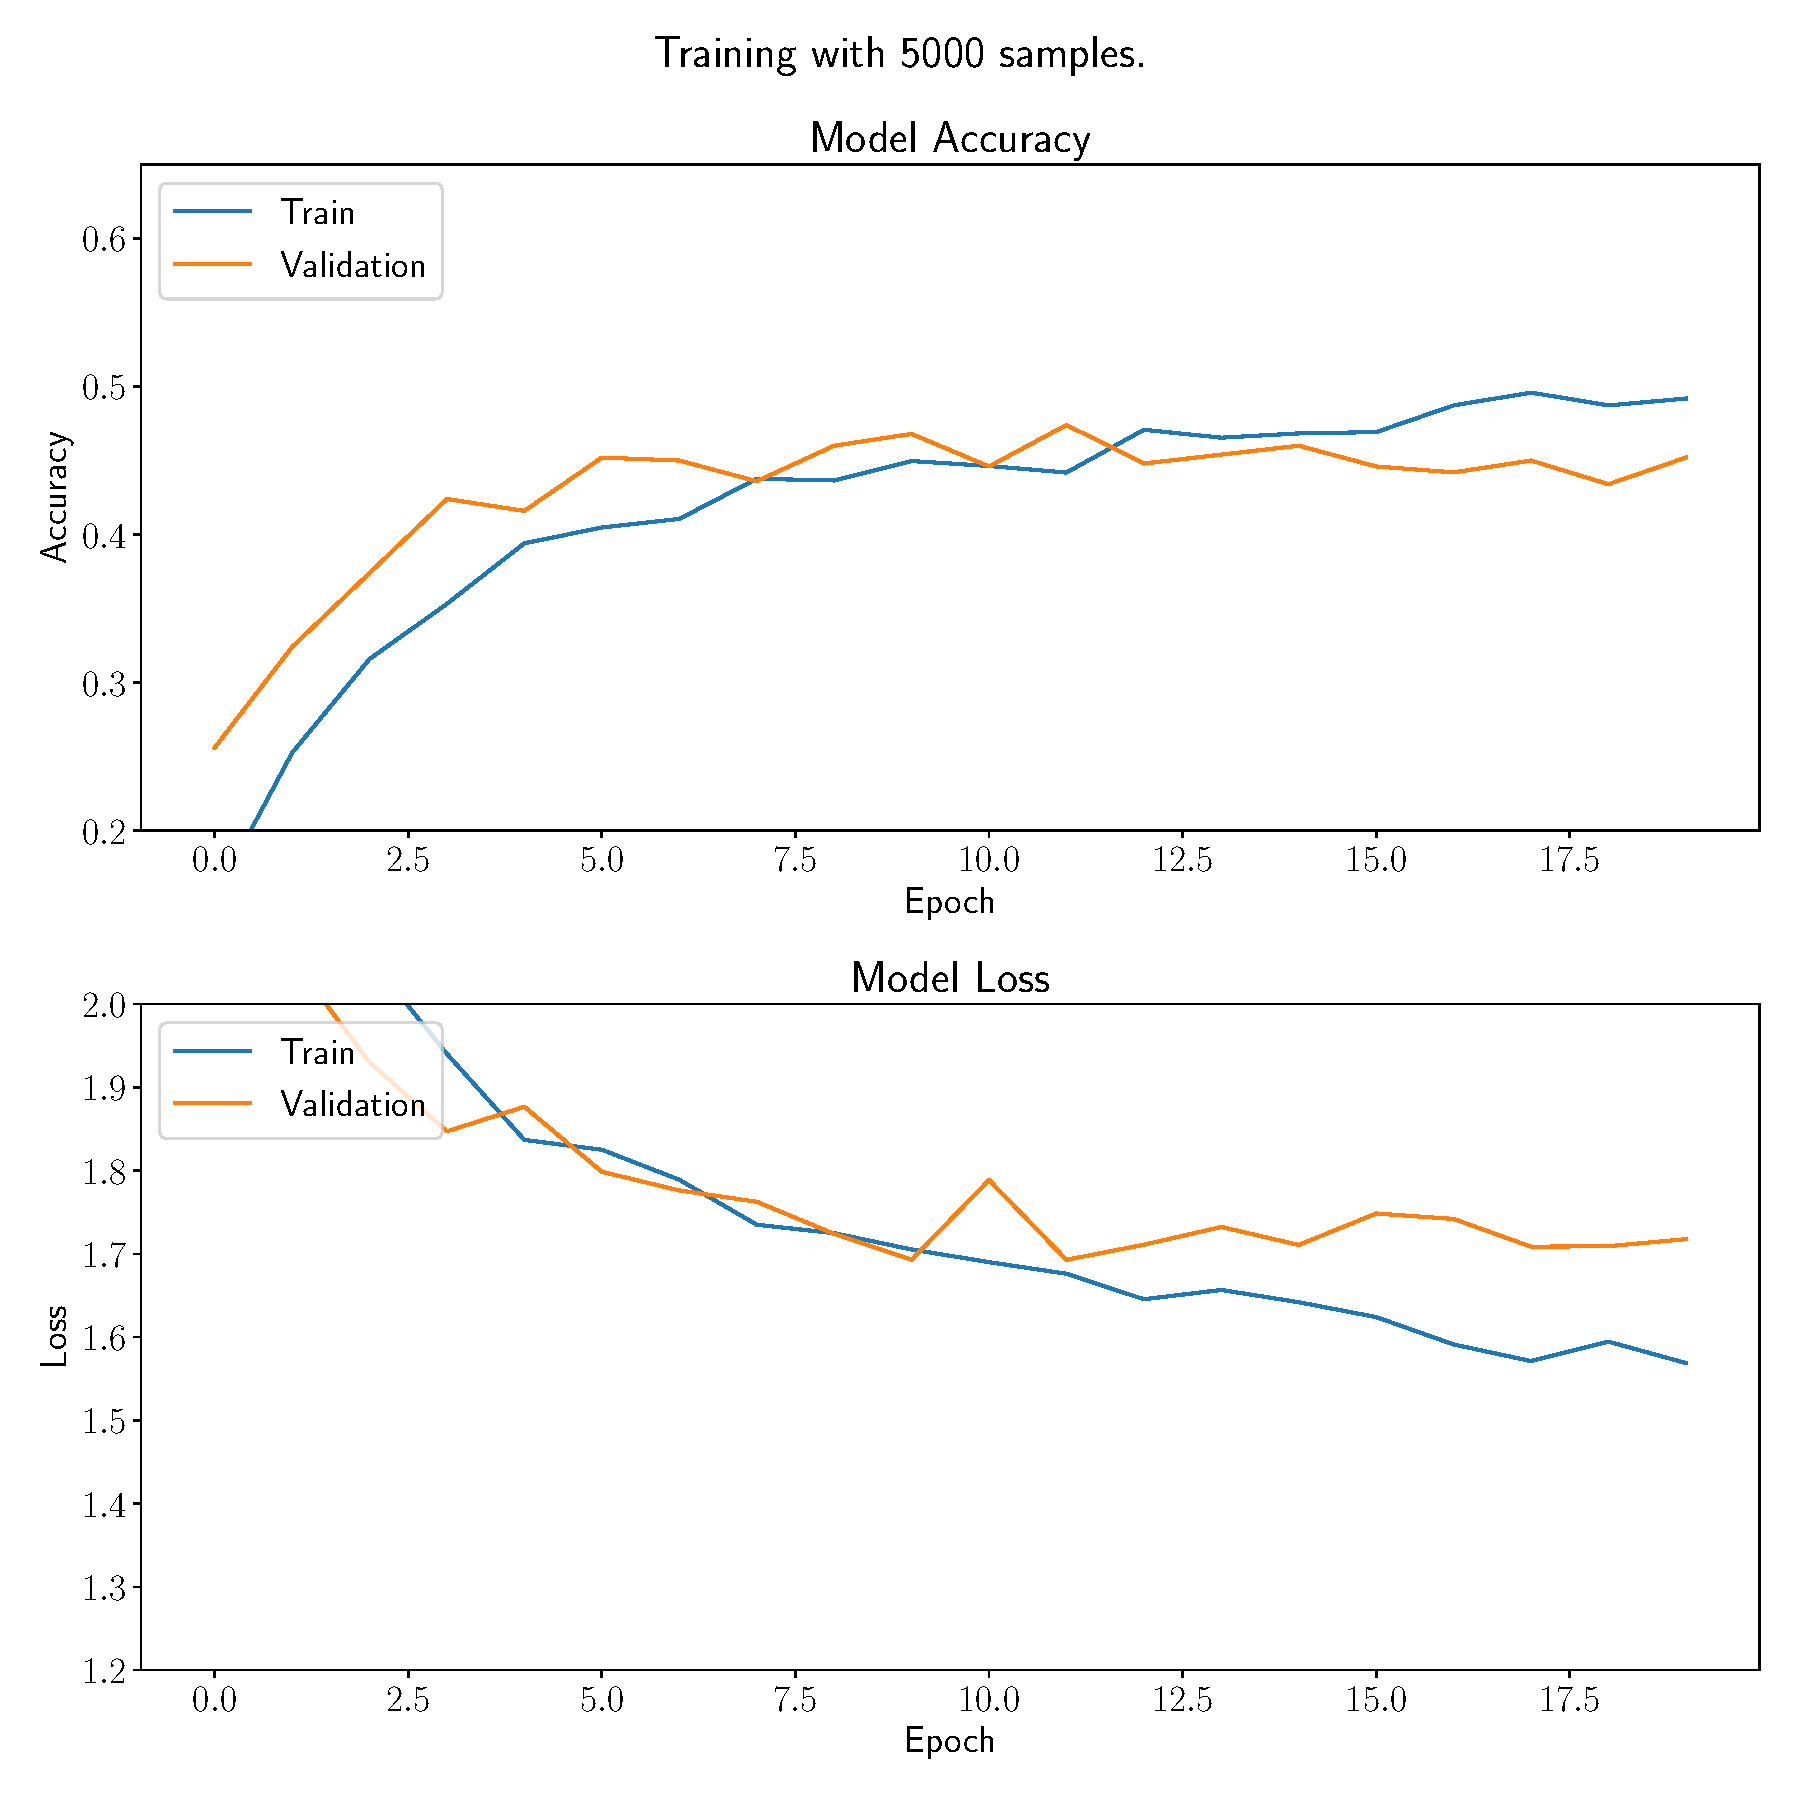
\includegraphics[width=0.49\textwidth]{exp/iibiii/5000.acc-loss.pdf}
    \par\end{centering}
    \caption{\label{fig:iibii-acc-loss}
    A comparison of accuracy/loss on training/test data from
    epochs 1 to 20 when trained on 5K training samples with $L_1=0.001$.}
\end{figure}

\subsection{(ii) (b) (iii)}
Figure \ref{fig:iibiii-acc-loss} presents plots of the `histories' of the training losses and accuracies on training/validation data
for a sequence of models trained on 5K, 10K, 20K, and 40K training samples.
Naturally, the model with most training data achievs the lowest loss and highest accuracy on the validation data.
For 5K training samples the gap between training and validatin scores starts to increase after about 10 epochs, indicating over-fitting.
In particular, by the 20th epoch the accuracy on the training data is higher than the accuracy on the validation data
and the loss on the training data is lower than the loss on the validatin data.
With 40K training samples there is a disimprovement at the 16th epoch, but the 17th, 18th, 19th and 20th epoch scores do not indicate
significant over-fitting.

The general reading we can take from Figure \ref{fig:iibiii-acc-loss} is that more training data allows us to train for more epochs without over-fitting, or without over-fitting as much.

\begin{figure}
    \begin{centering}
        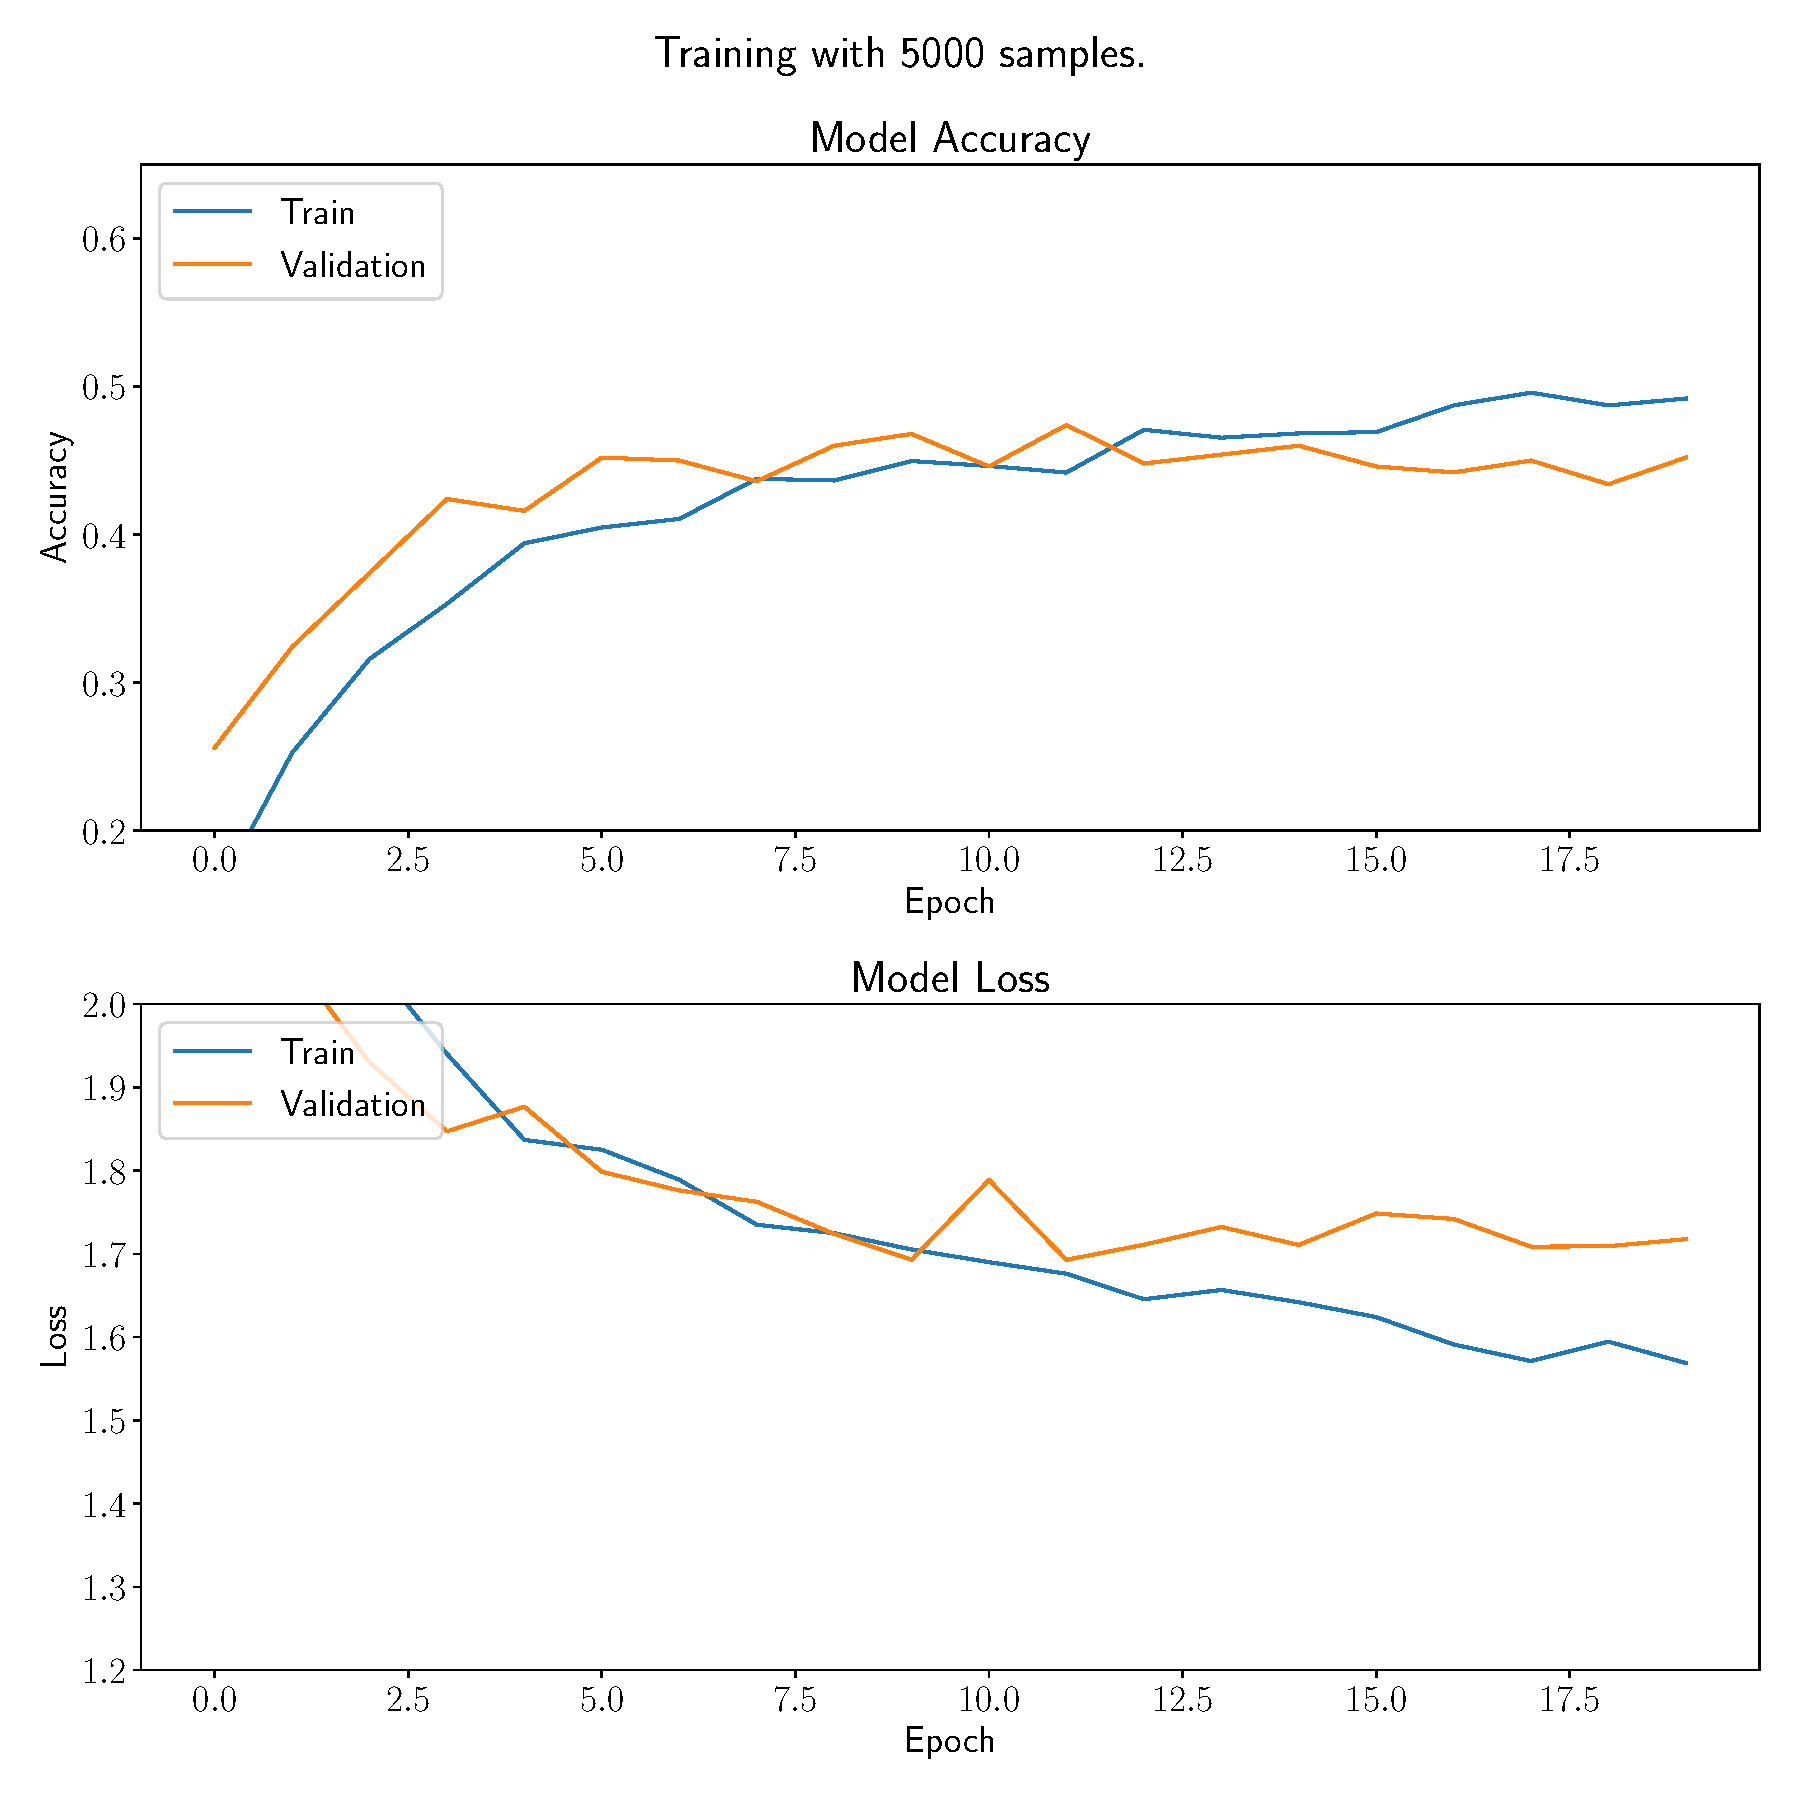
\includegraphics[width=0.49\textwidth]{exp/iibiii/5000.acc-loss.pdf}
        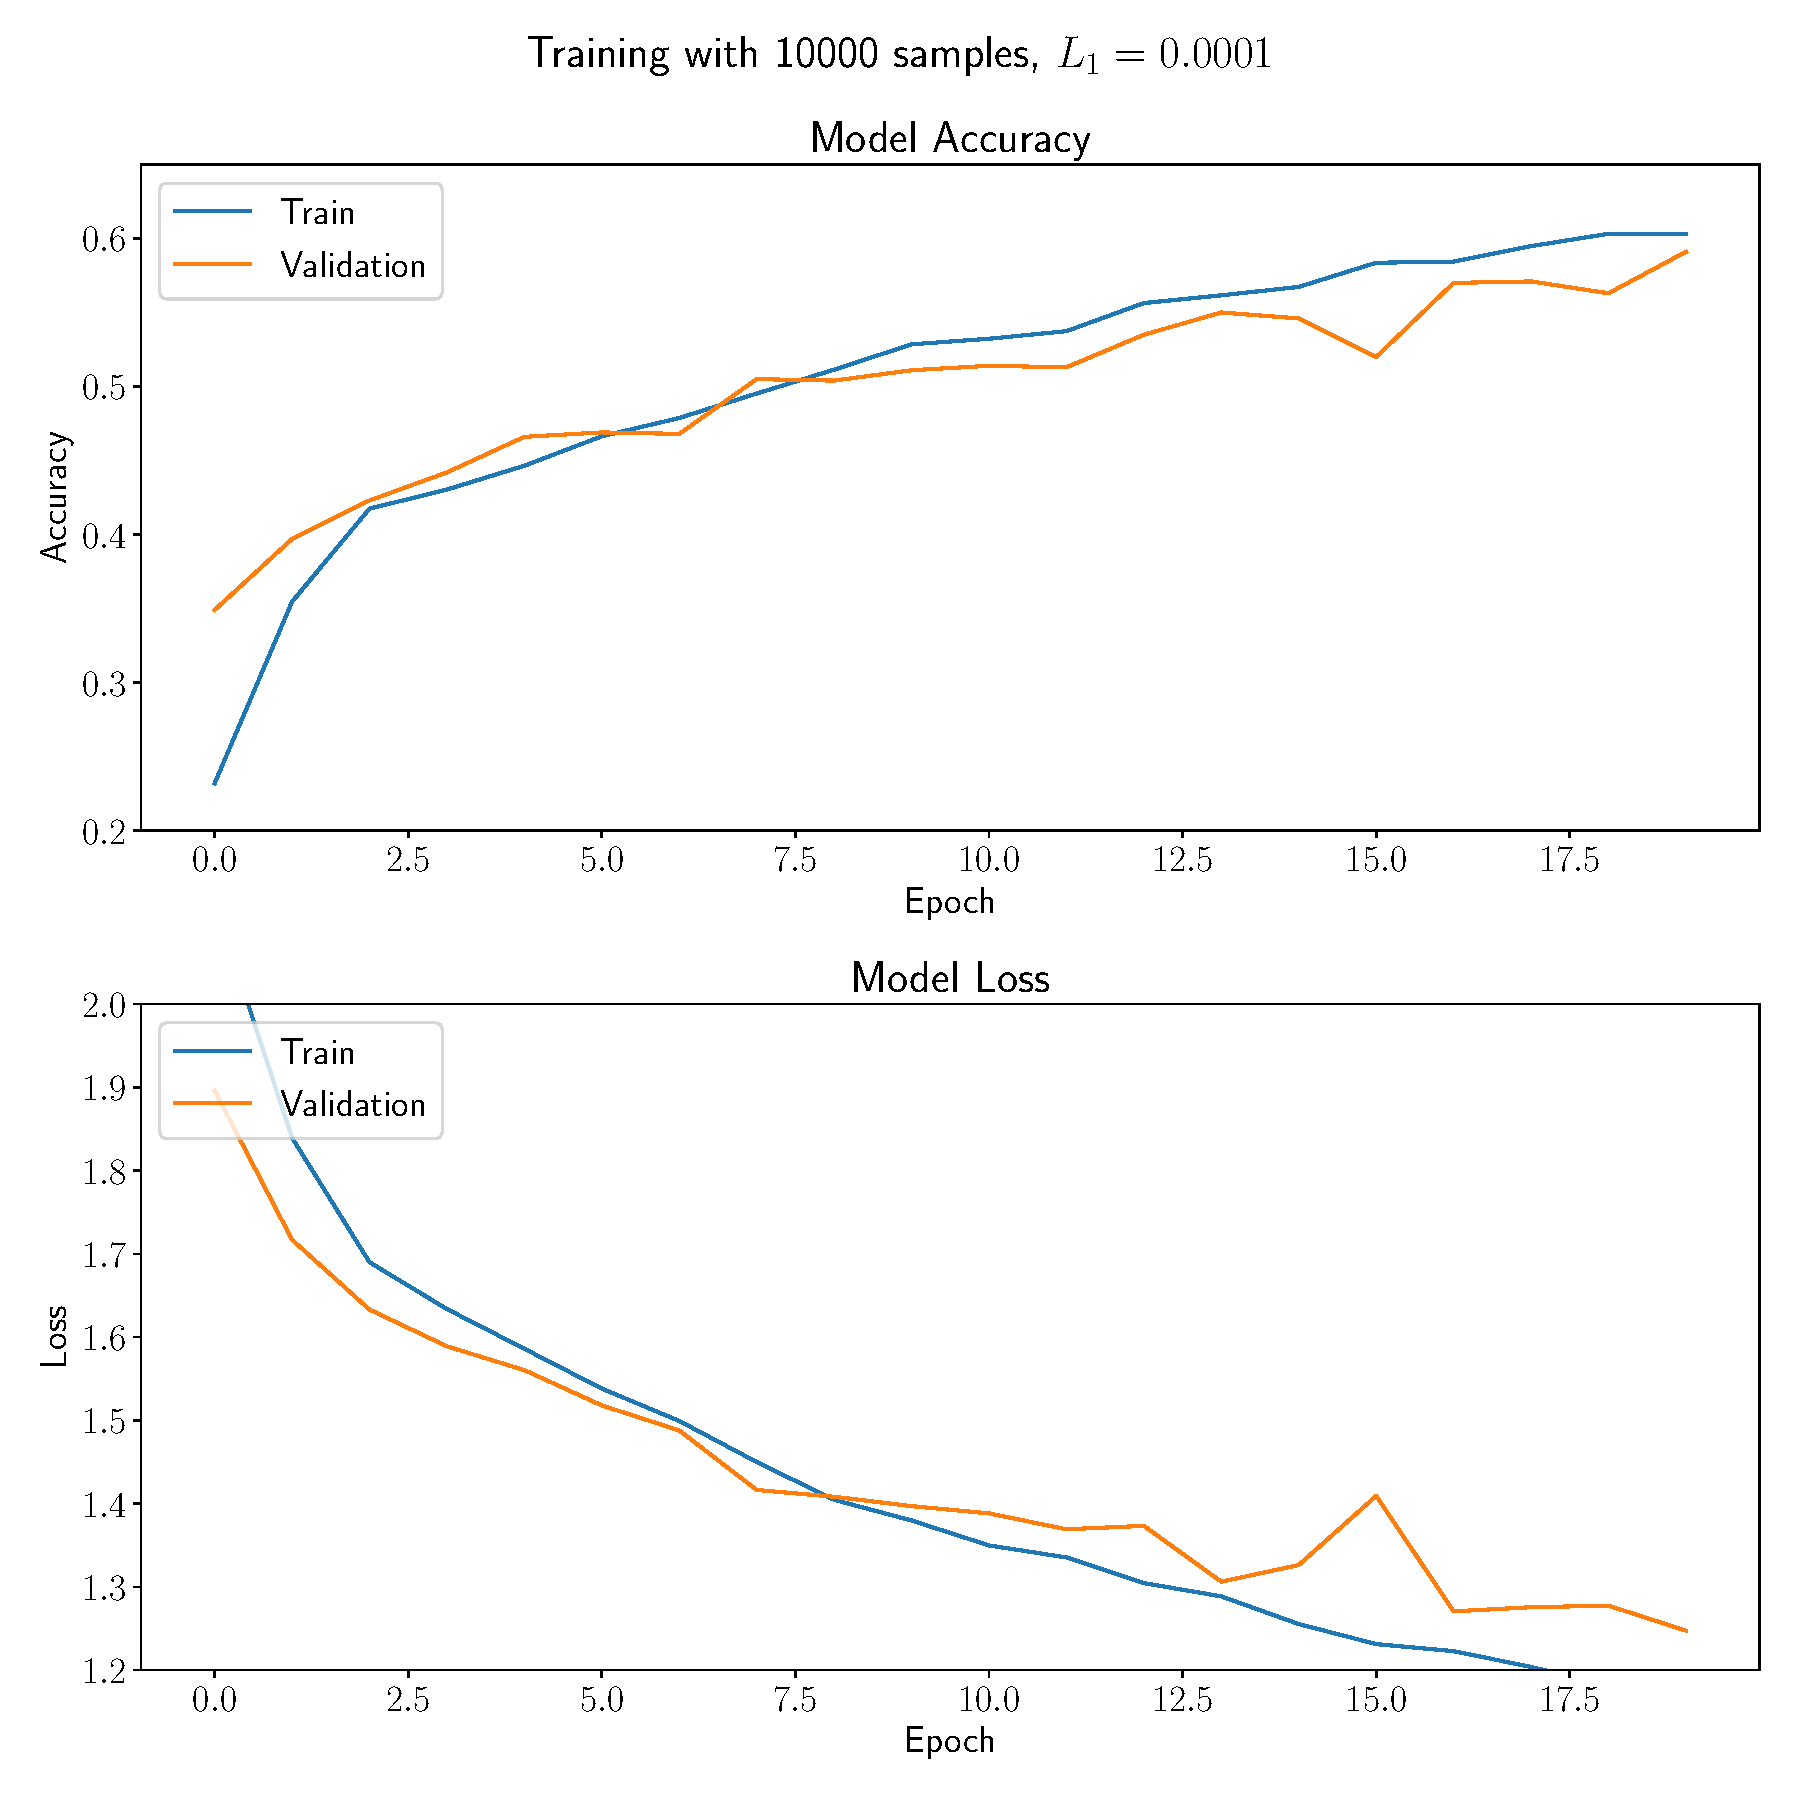
\includegraphics[width=0.49\textwidth]{exp/iibiii/10000.acc-loss.pdf}
    \par\end{centering}
    \begin{centering}
        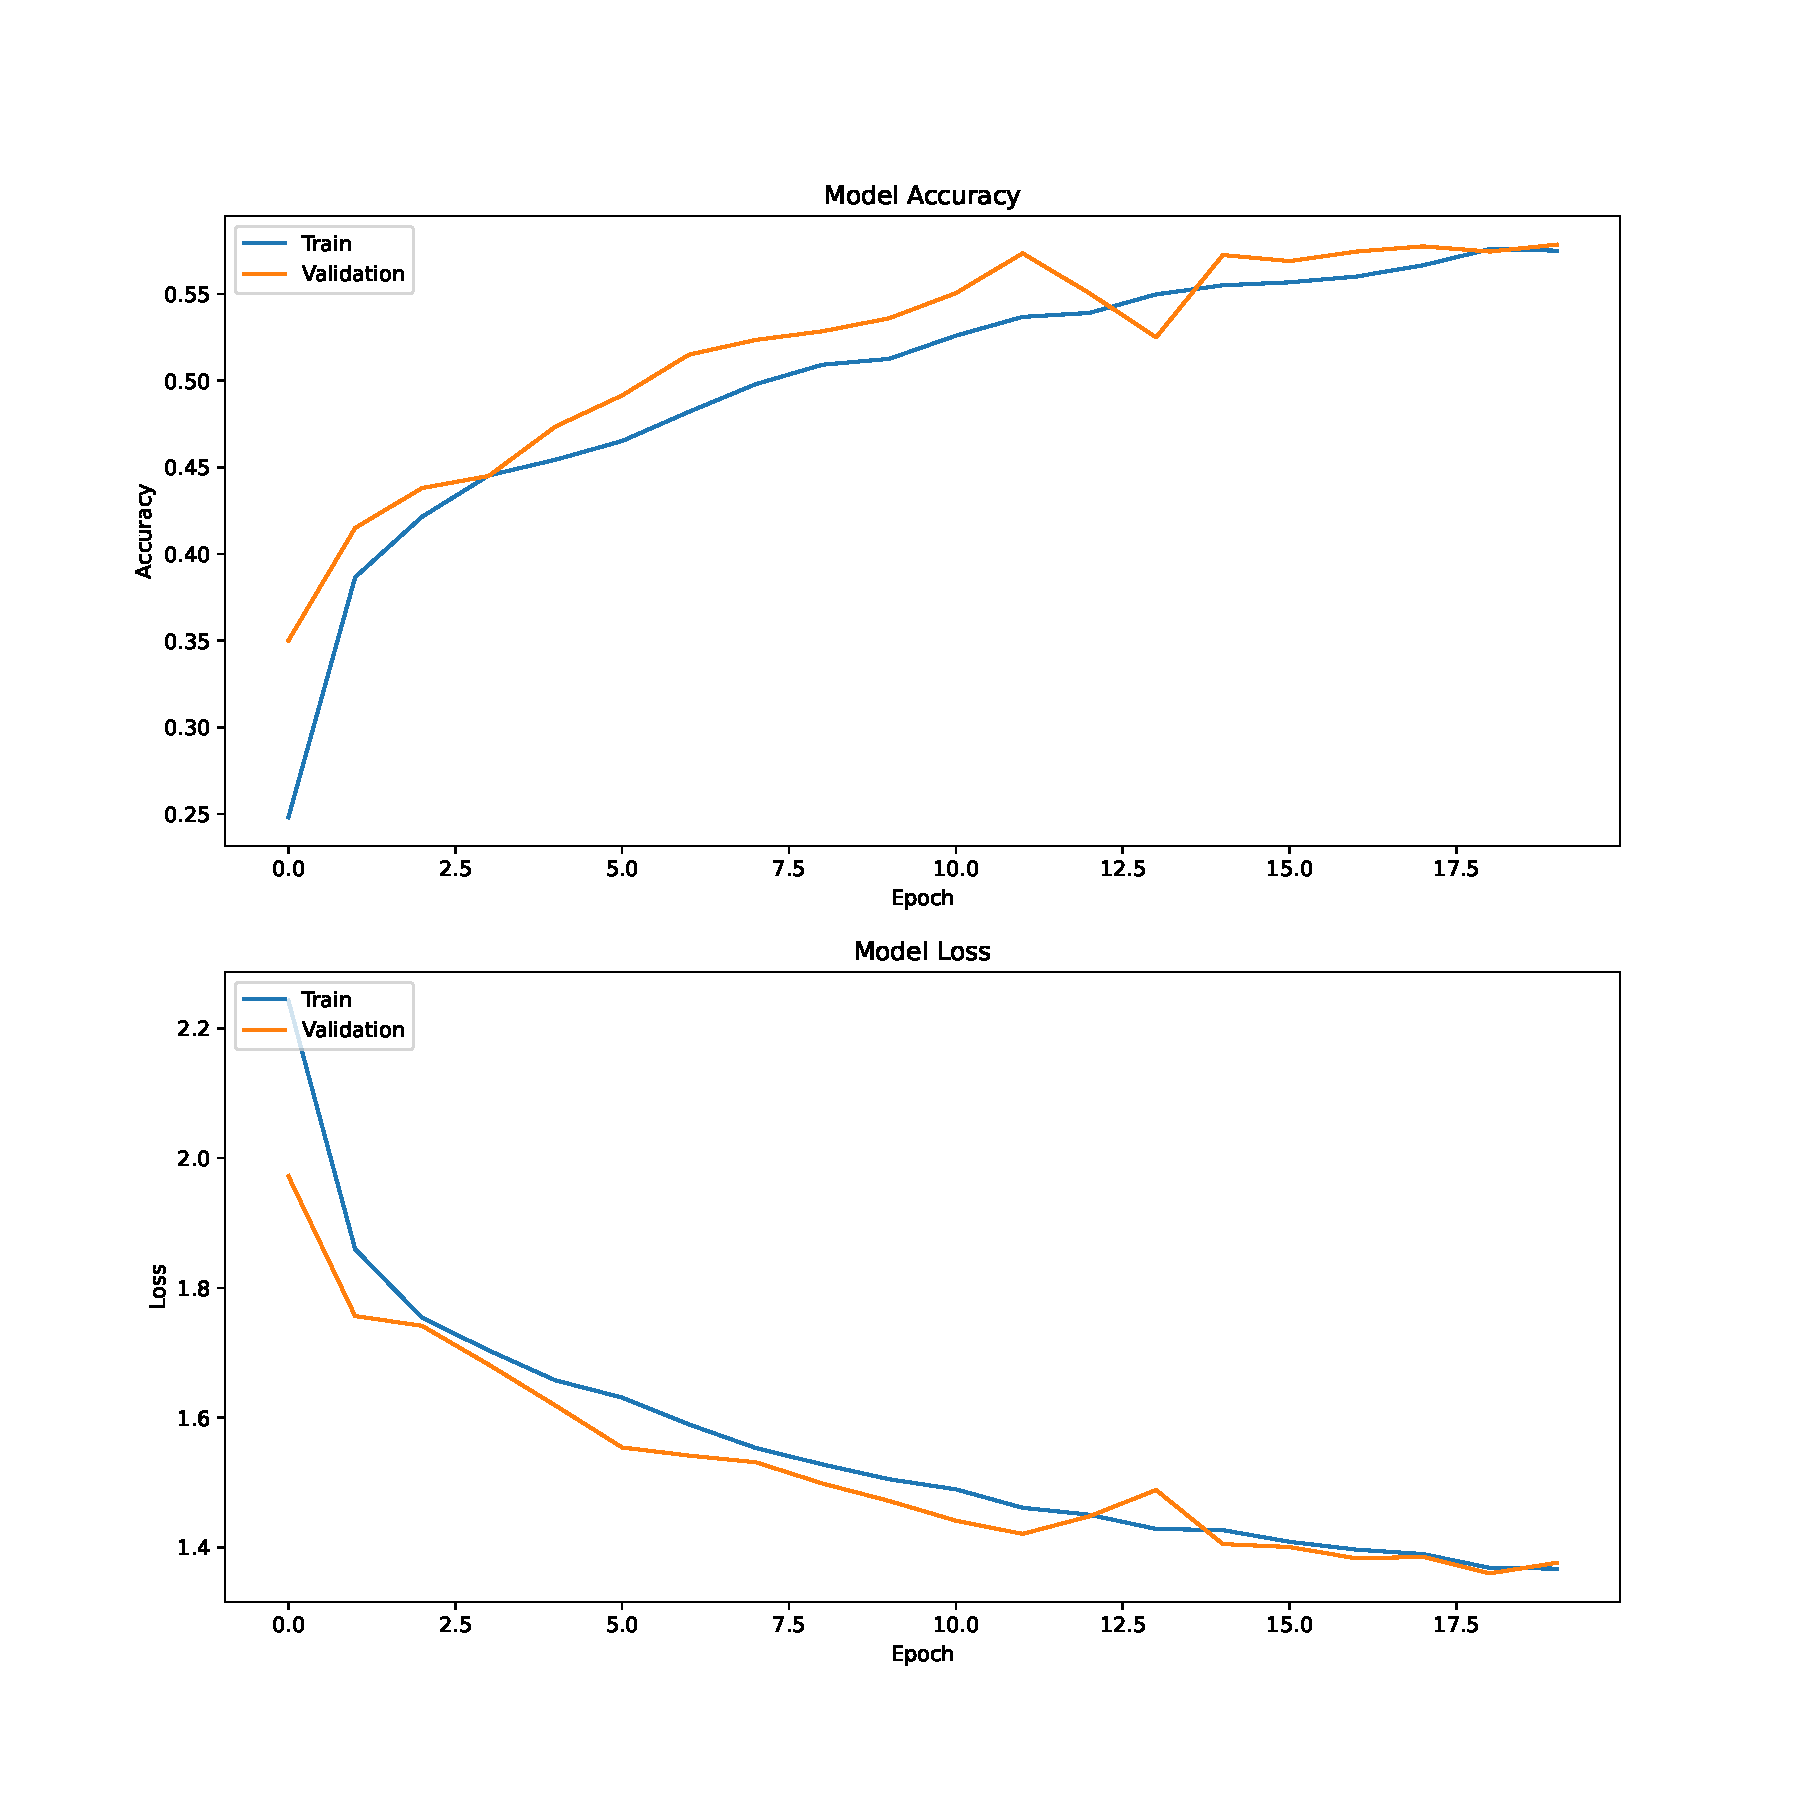
\includegraphics[width=0.49\textwidth]{exp/iibiii/20000.acc-loss.pdf}
        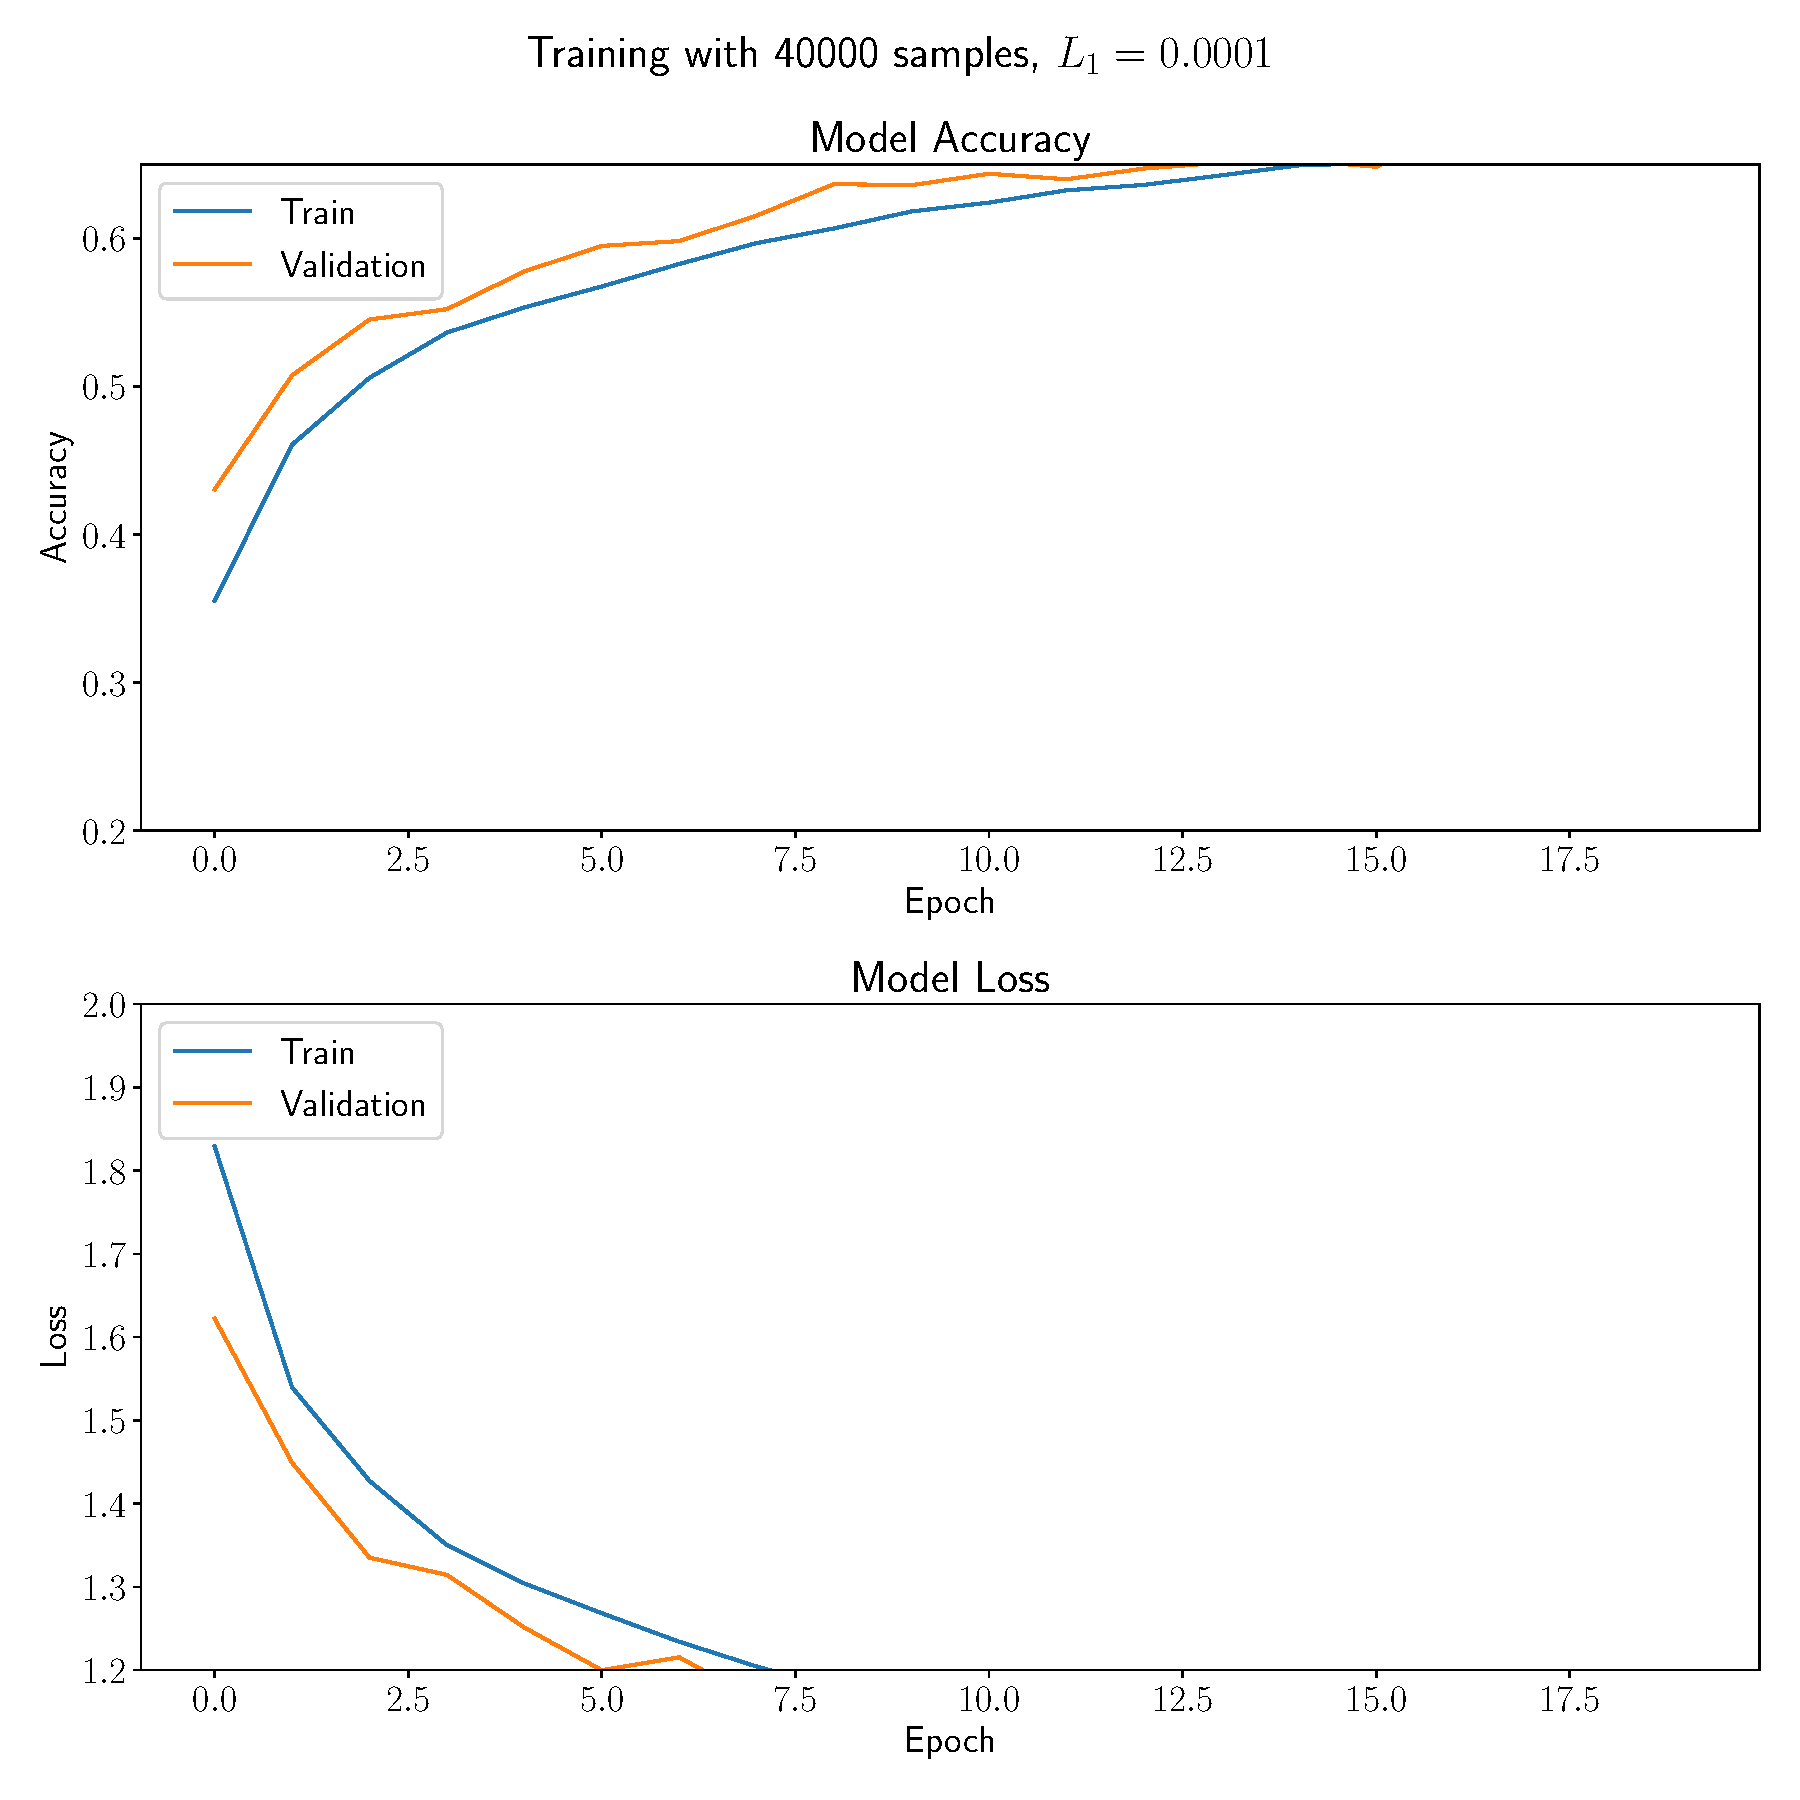
\includegraphics[width=0.49\textwidth]{exp/iibiii/40000.acc-loss.pdf}
    \par\end{centering}
    \caption{\label{fig:iibiii-acc-loss}
    A comparison of accuracy/loss on training/test data from
    epochs 1 to 20 for different quantities
    of training data, 5K, 10K, 20K and 40K.  Each model is trained with $L_1=0.001$.}
\end{figure}

\begin{figure}
    \begin{centering}
        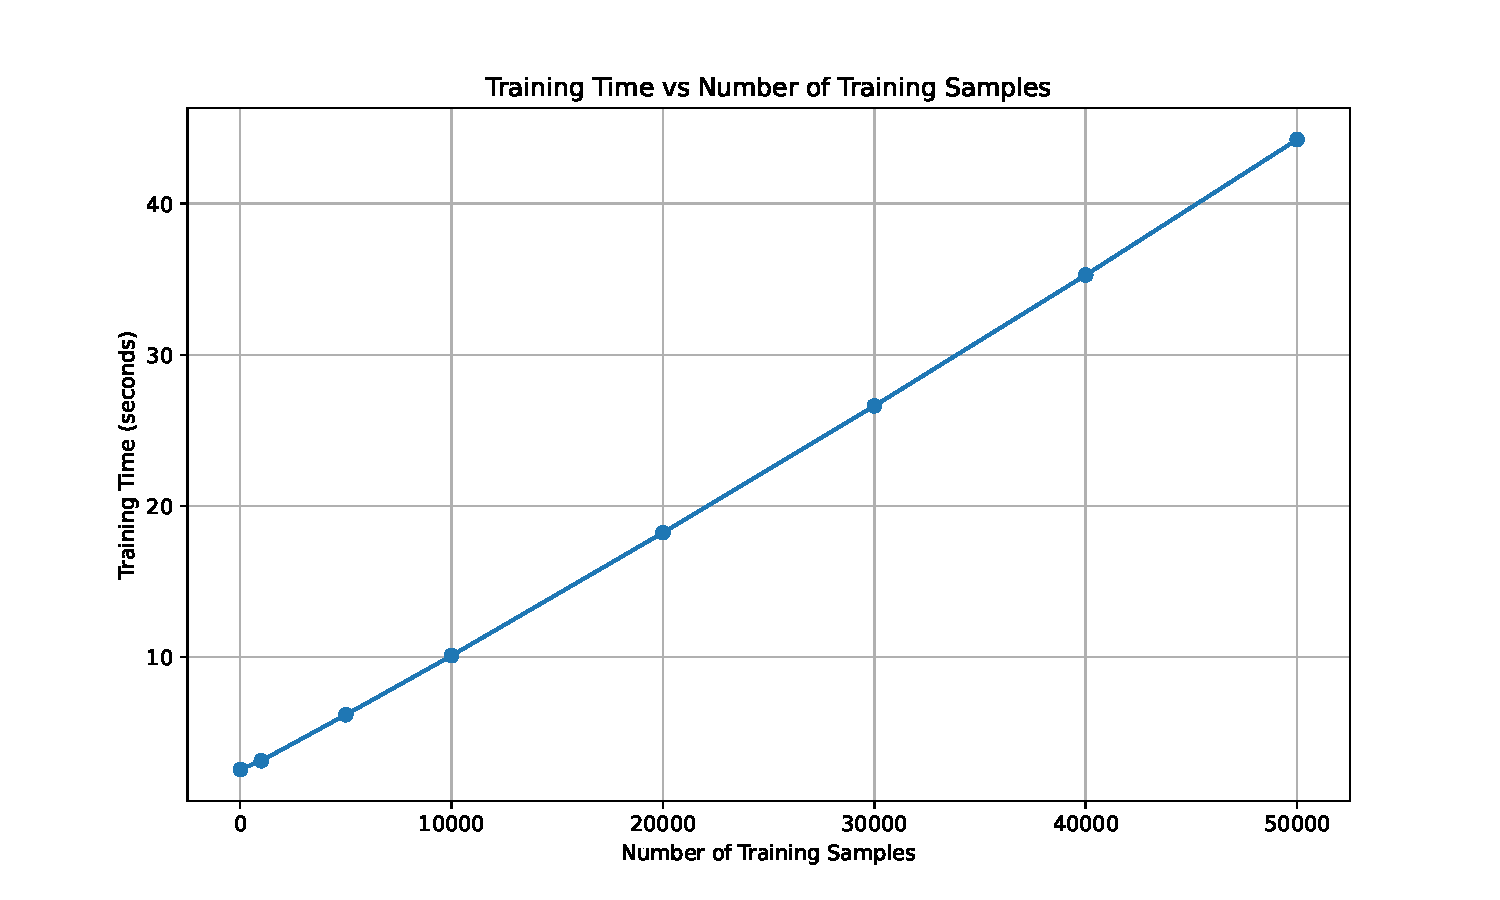
\includegraphics[width=0.5\textwidth]{exp/iibiii/time.pdf}
    \par\end{centering}
    \caption{\label{fig:timing}The amount of time needed to train the ConvNet for 20 epochs is 
    plotted against thet number of training samples used. The relationship is linear.}
\end{figure}

\subsection{(ii) (b) (iv)}
Figure \ref{fig:iibiv-acc-loss} presents plots of the `histories' of the training losses and accuracies on training/validation data
for a sequence of models with $L_1\in \{ 0.0,0.00001,0.01,100 \}$.

After 20 epochs the model with $L_1=0.00001$ had a train loss below val loss,
and train accuracy above val accuracy,
which indicates over-fitting,
but the model trained with $L_1=0.01$ exhibits an opposite pattern,
where val score is better than thet train score.
However, while the model with $L_1=0.00001$ shows more signs of being fitted too closely to the training data,
the accuracy of the model on validation set is better than the accuracy of the more regularized model, $L_1=0.01$.


\begin{figure}
    \begin{centering}
        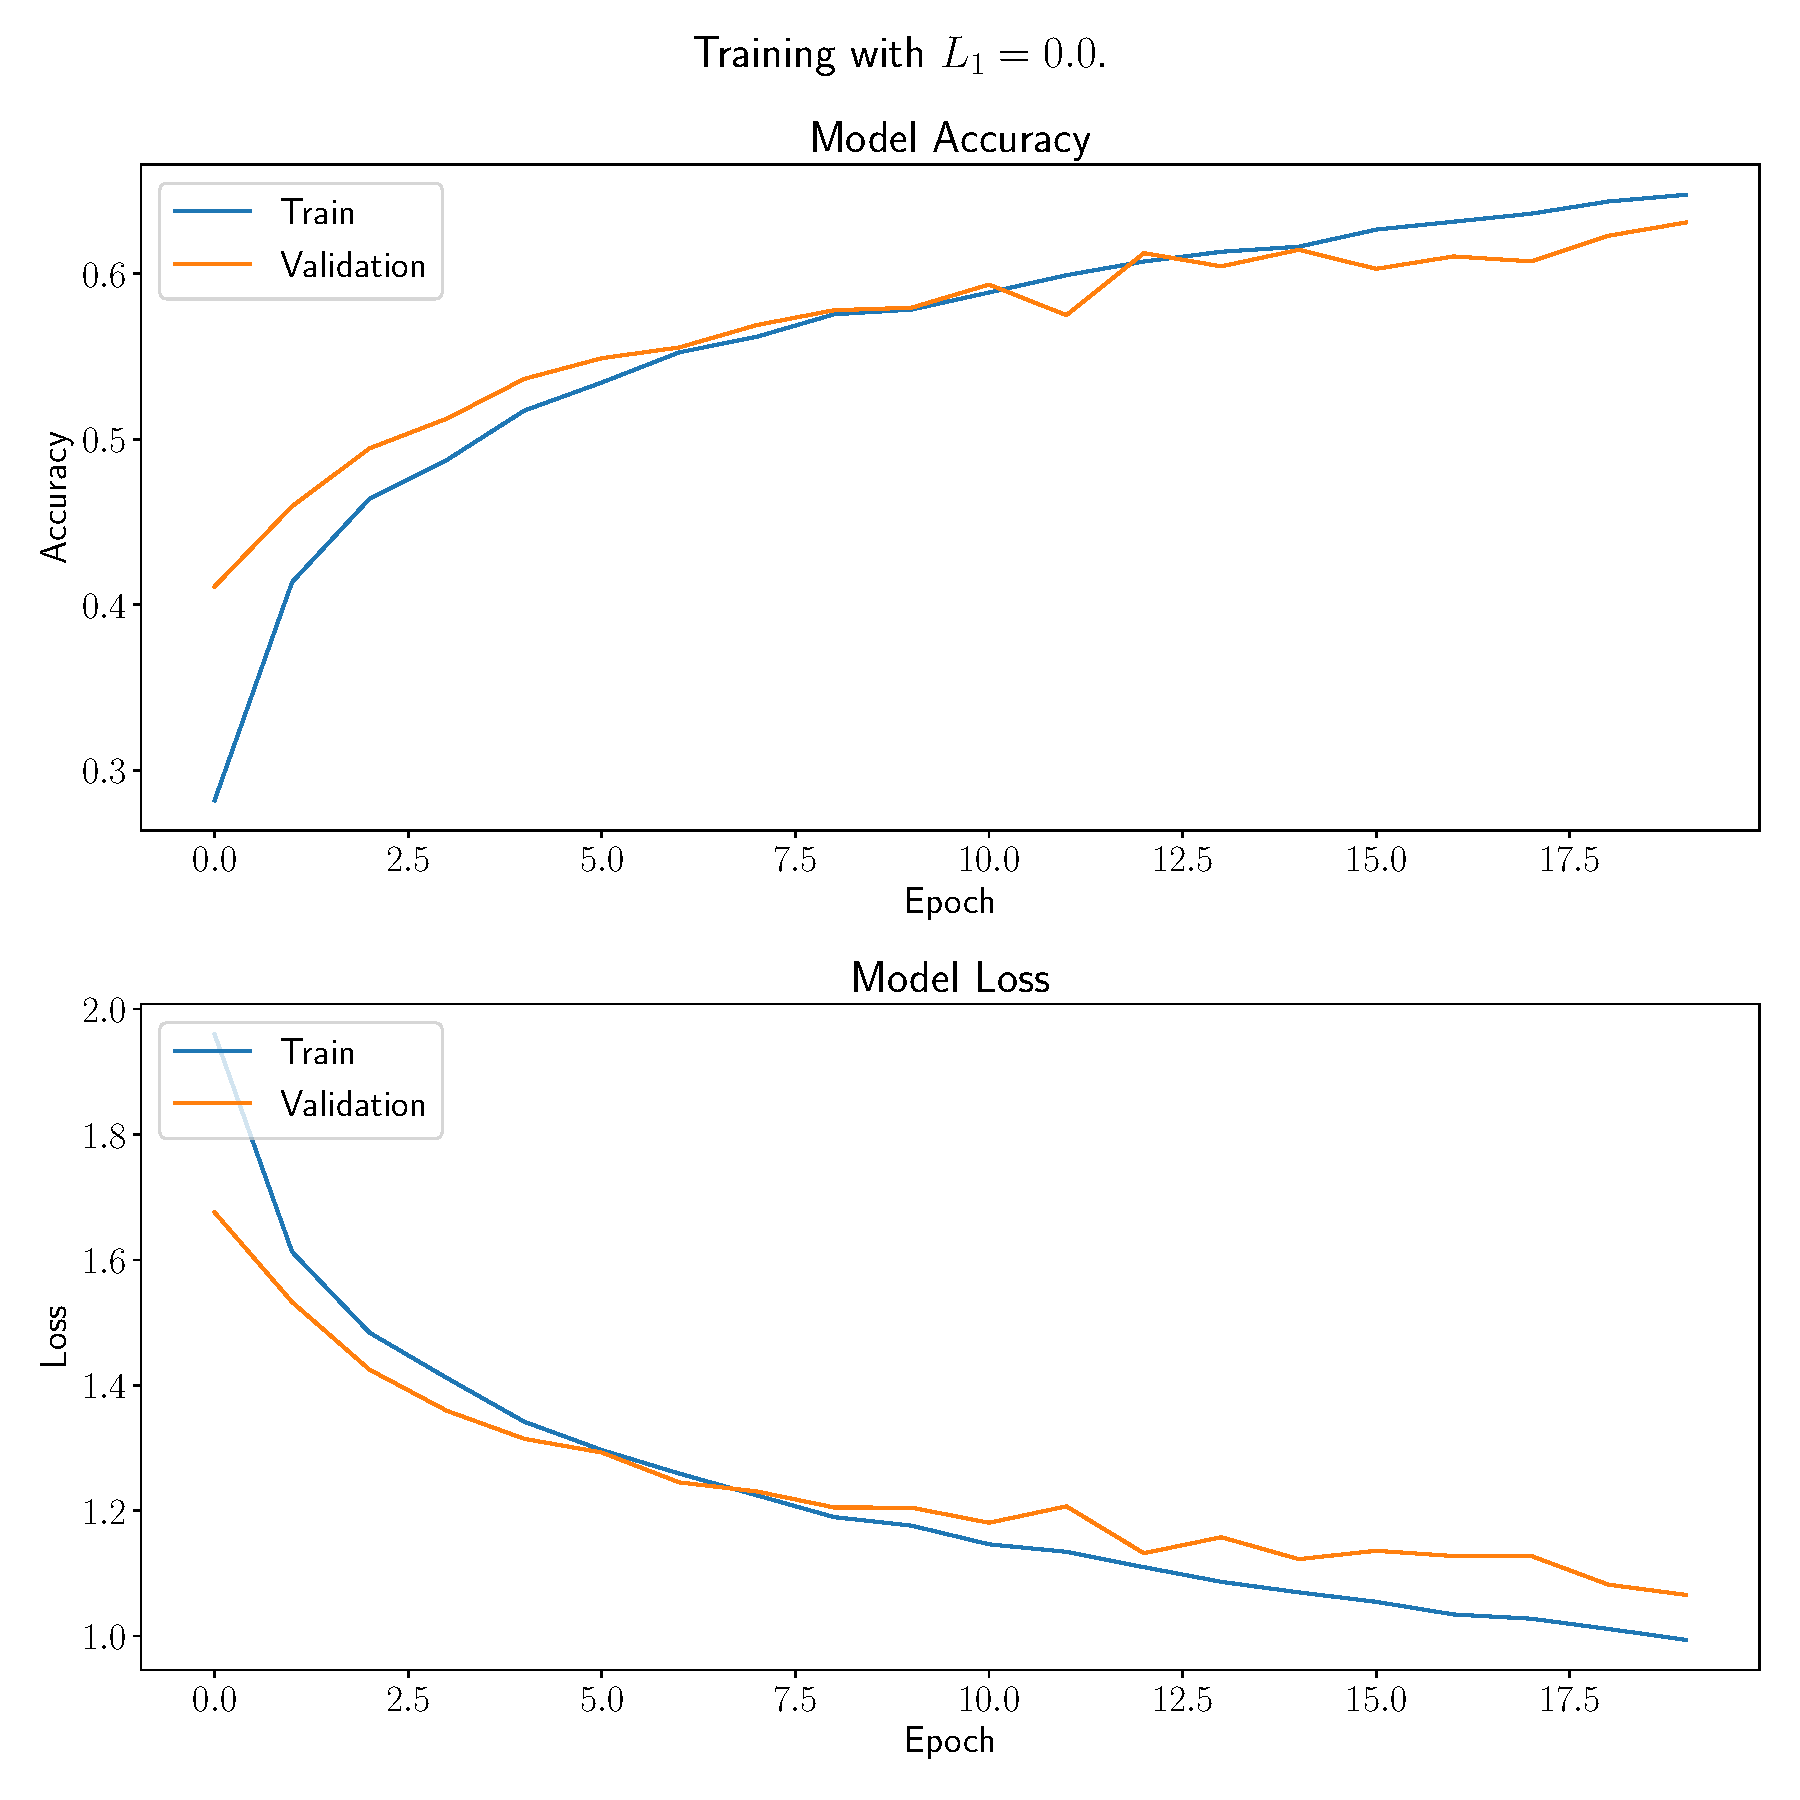
\includegraphics[width=0.49\textwidth]{exp/iibiv/0.0.acc-loss.pdf}
        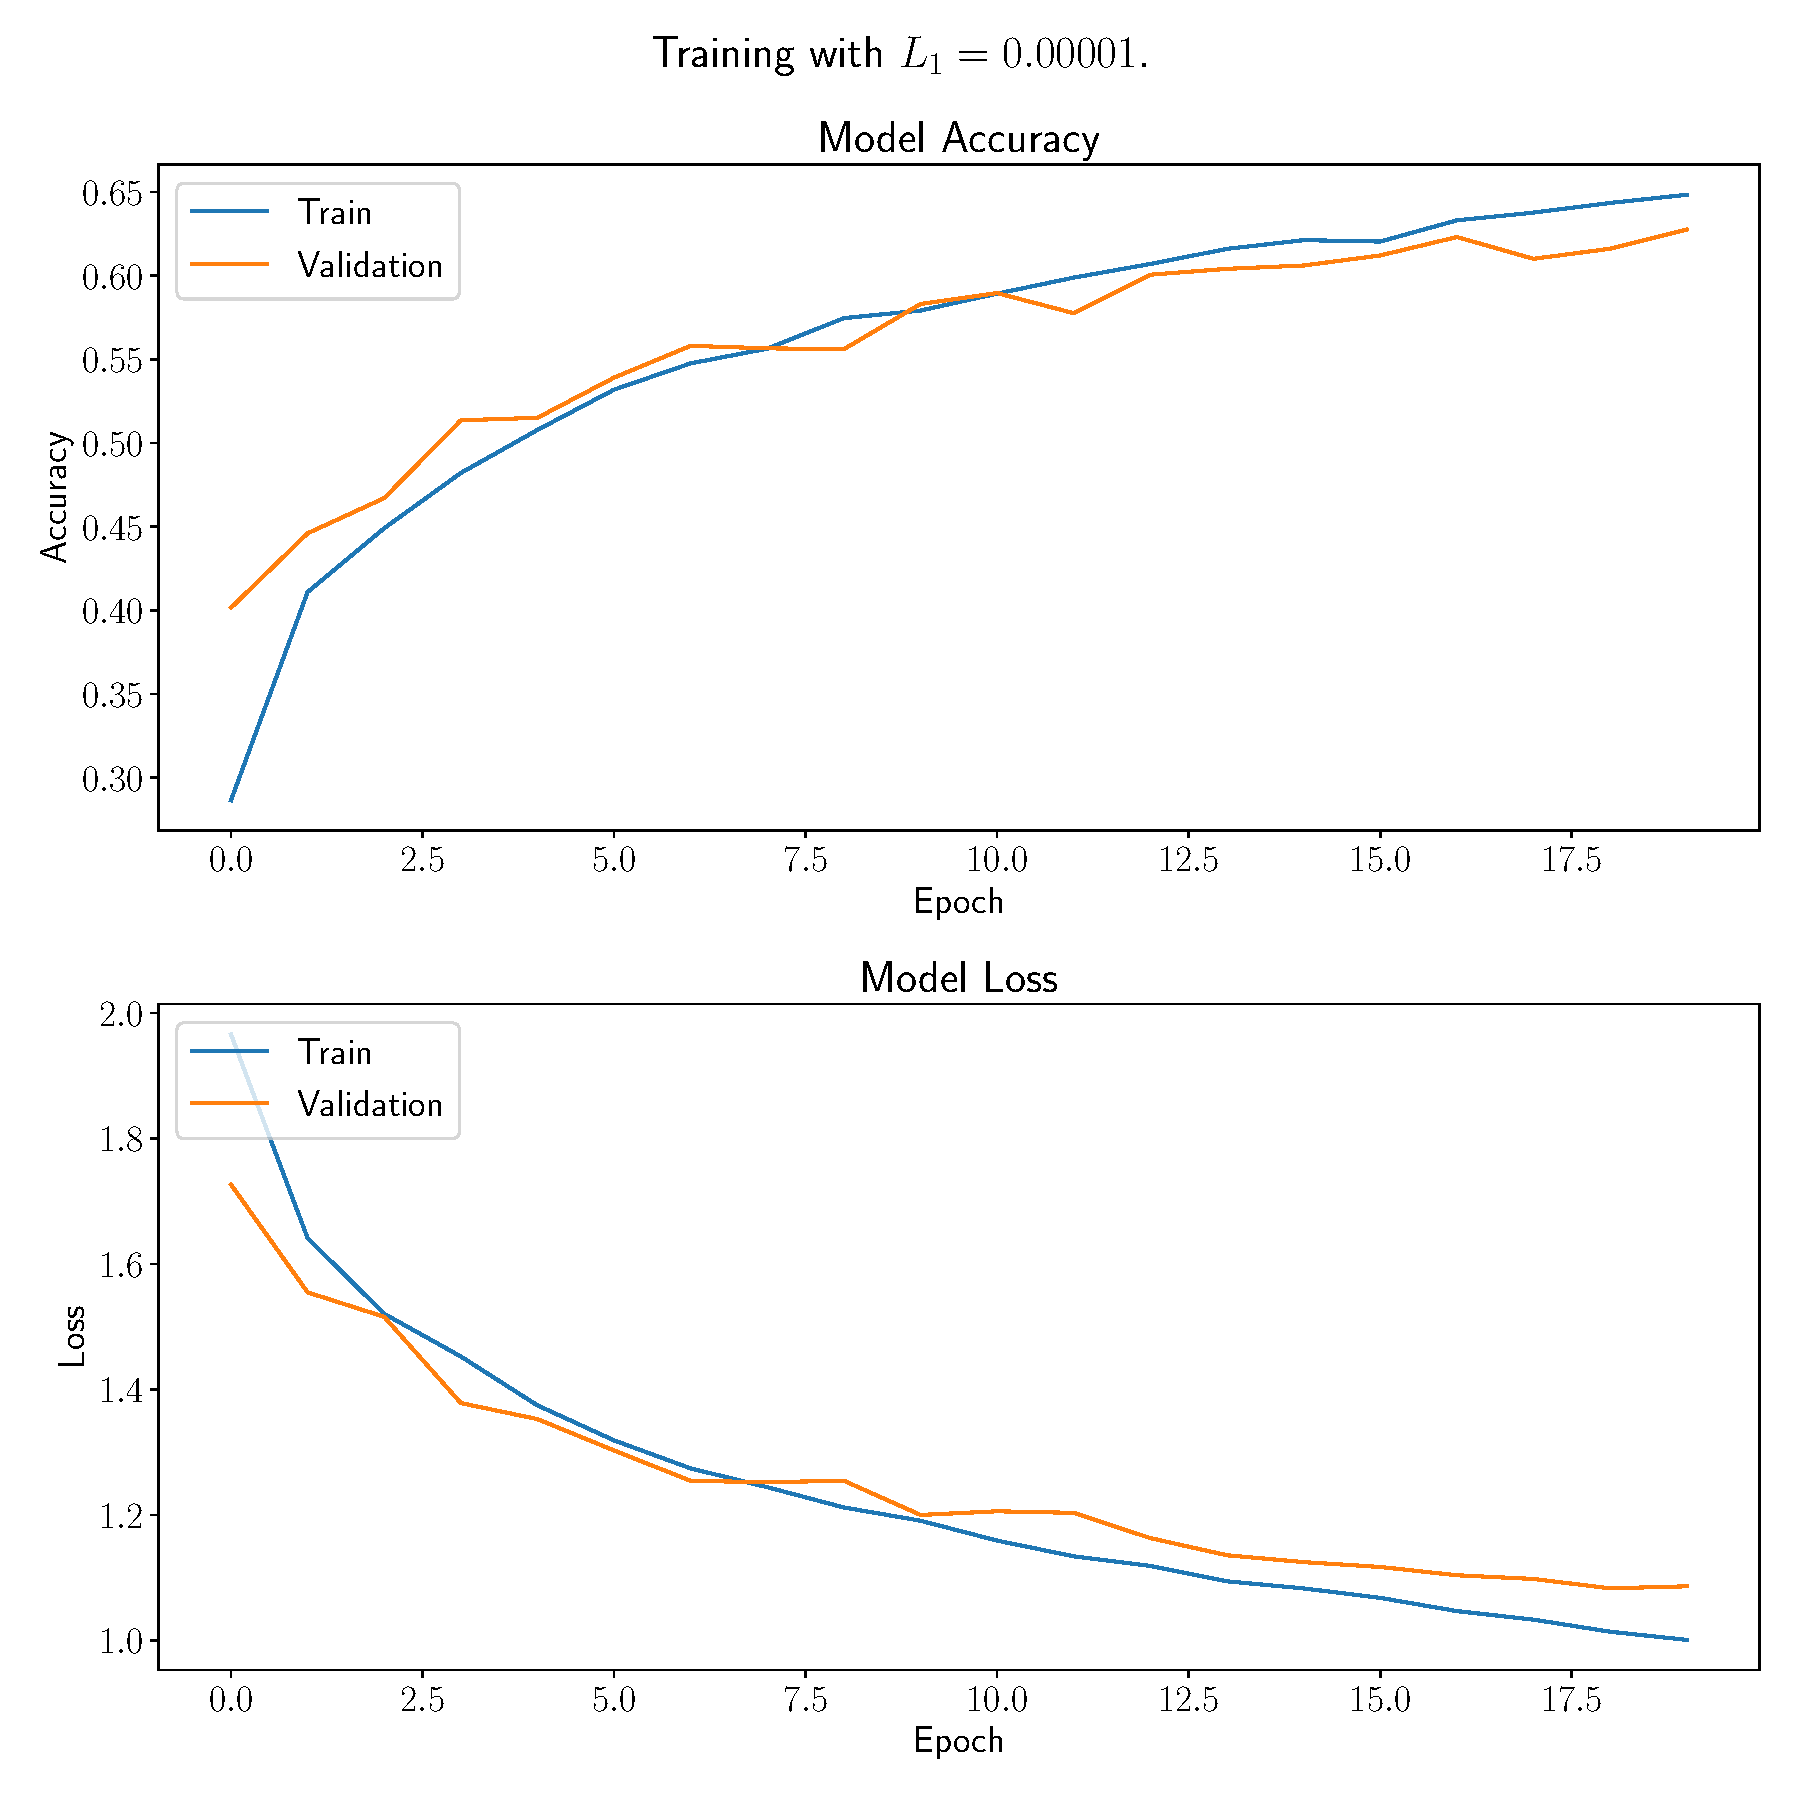
\includegraphics[width=0.49\textwidth]{exp/iibiv/0.00001.acc-loss.pdf}
    \par\end{centering}
    \begin{centering}
        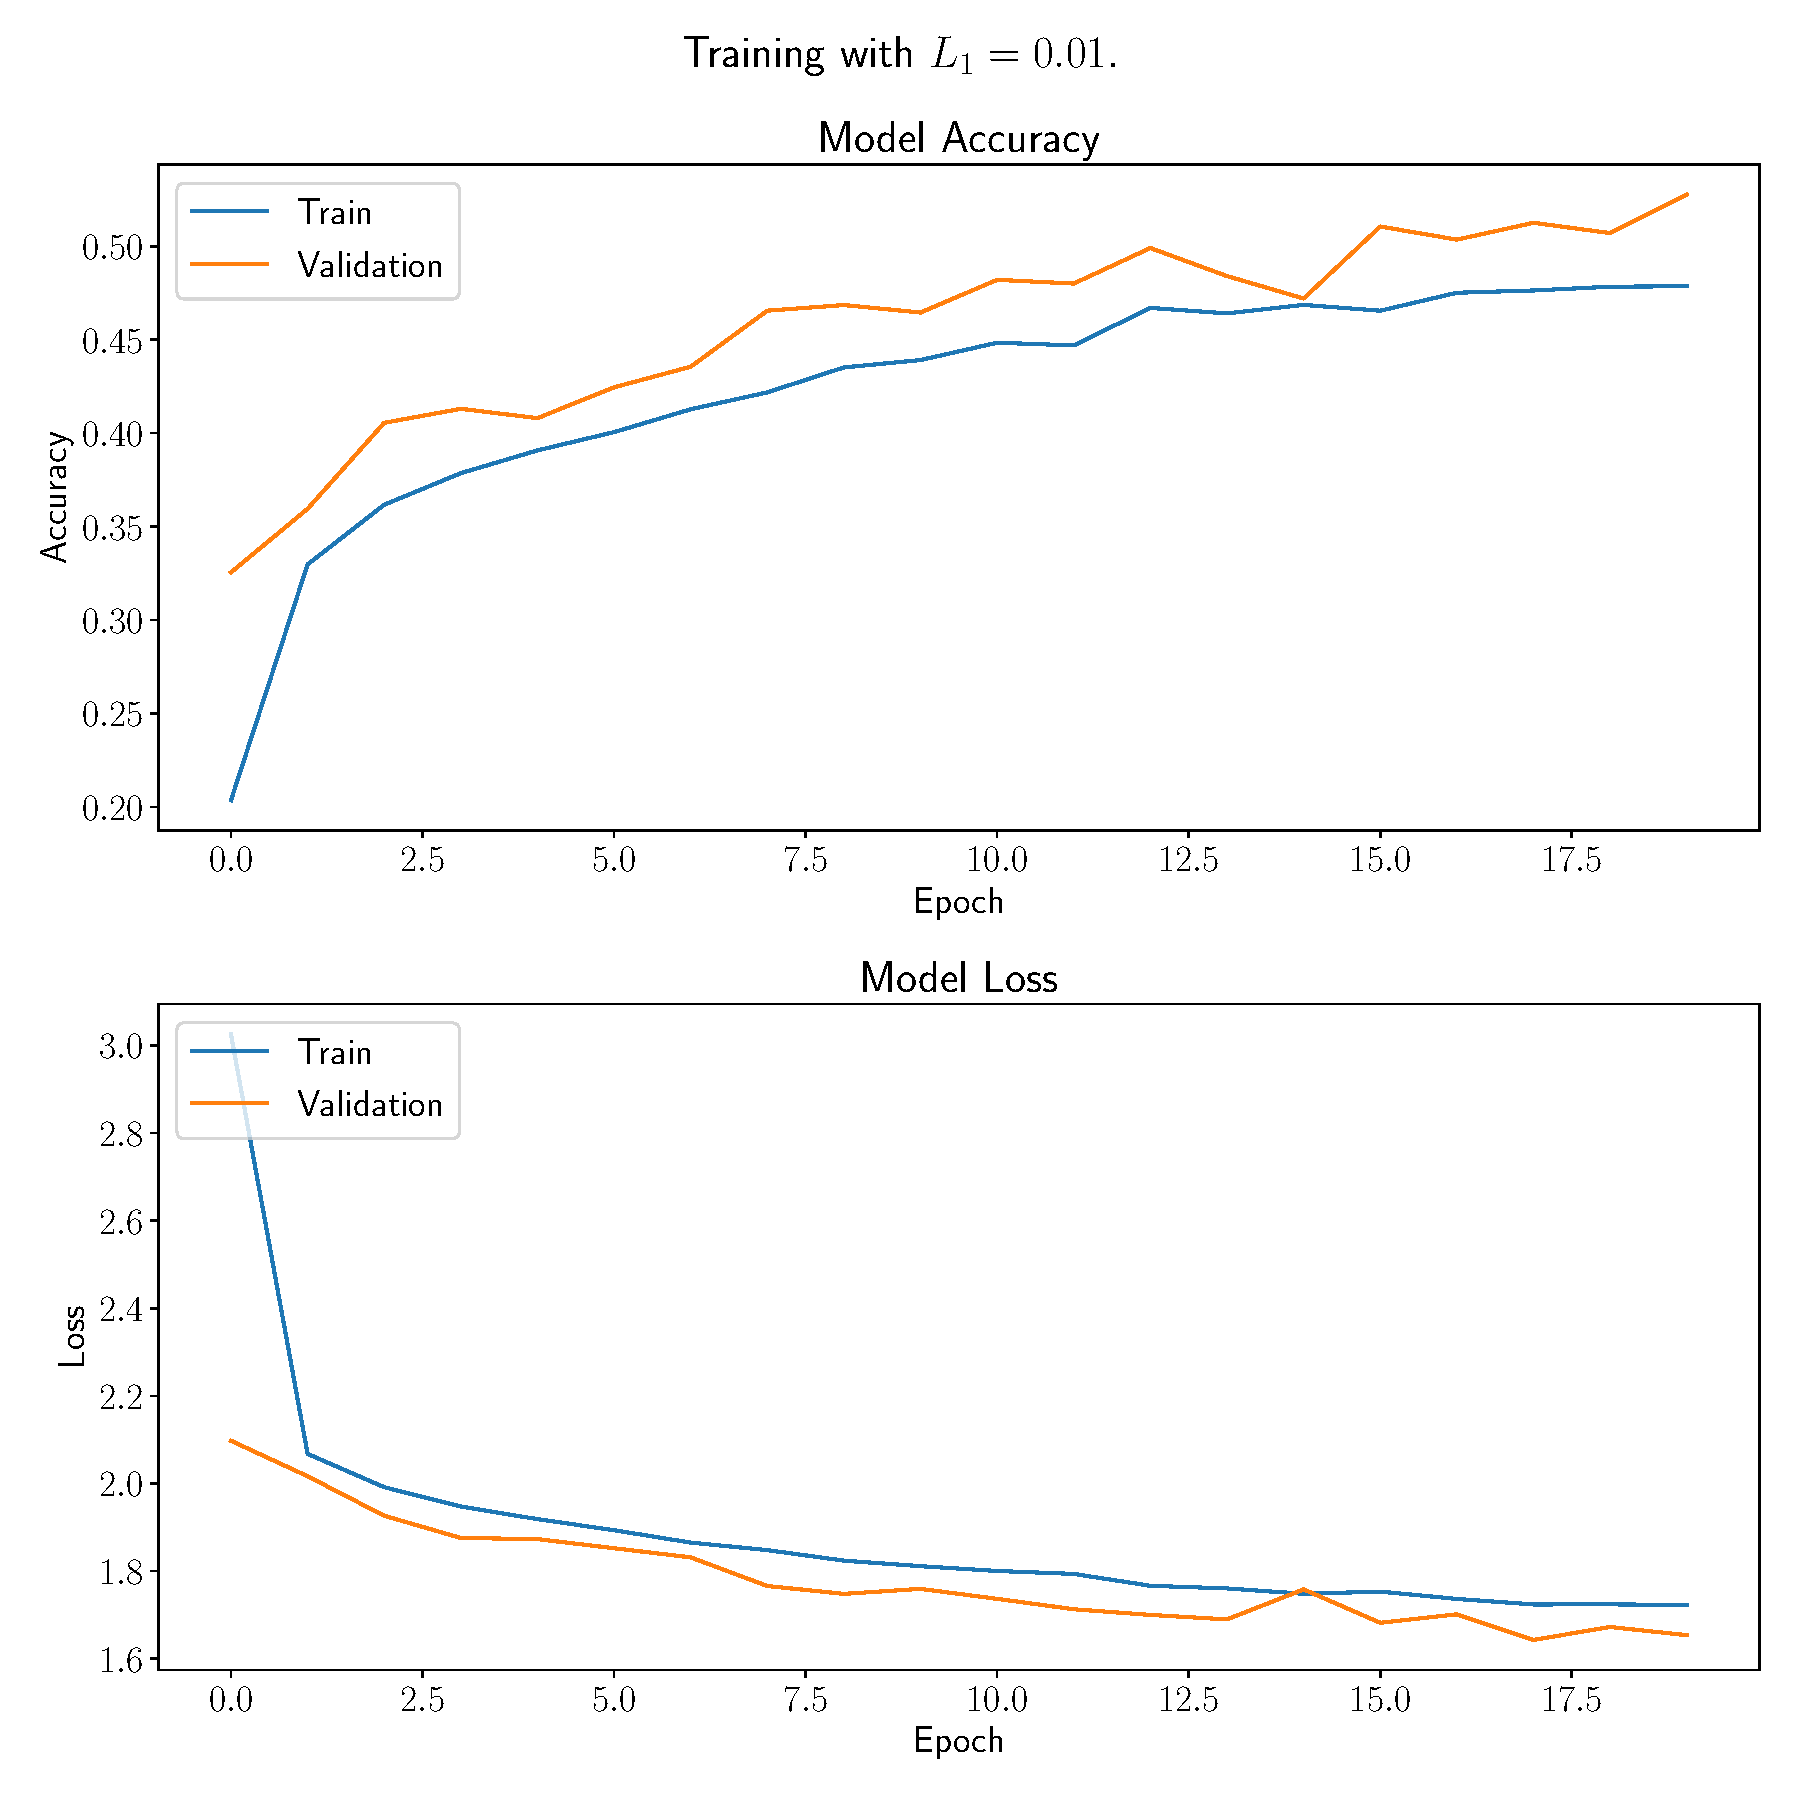
\includegraphics[width=0.49\textwidth]{exp/iibiv/0.01.acc-loss.pdf}
        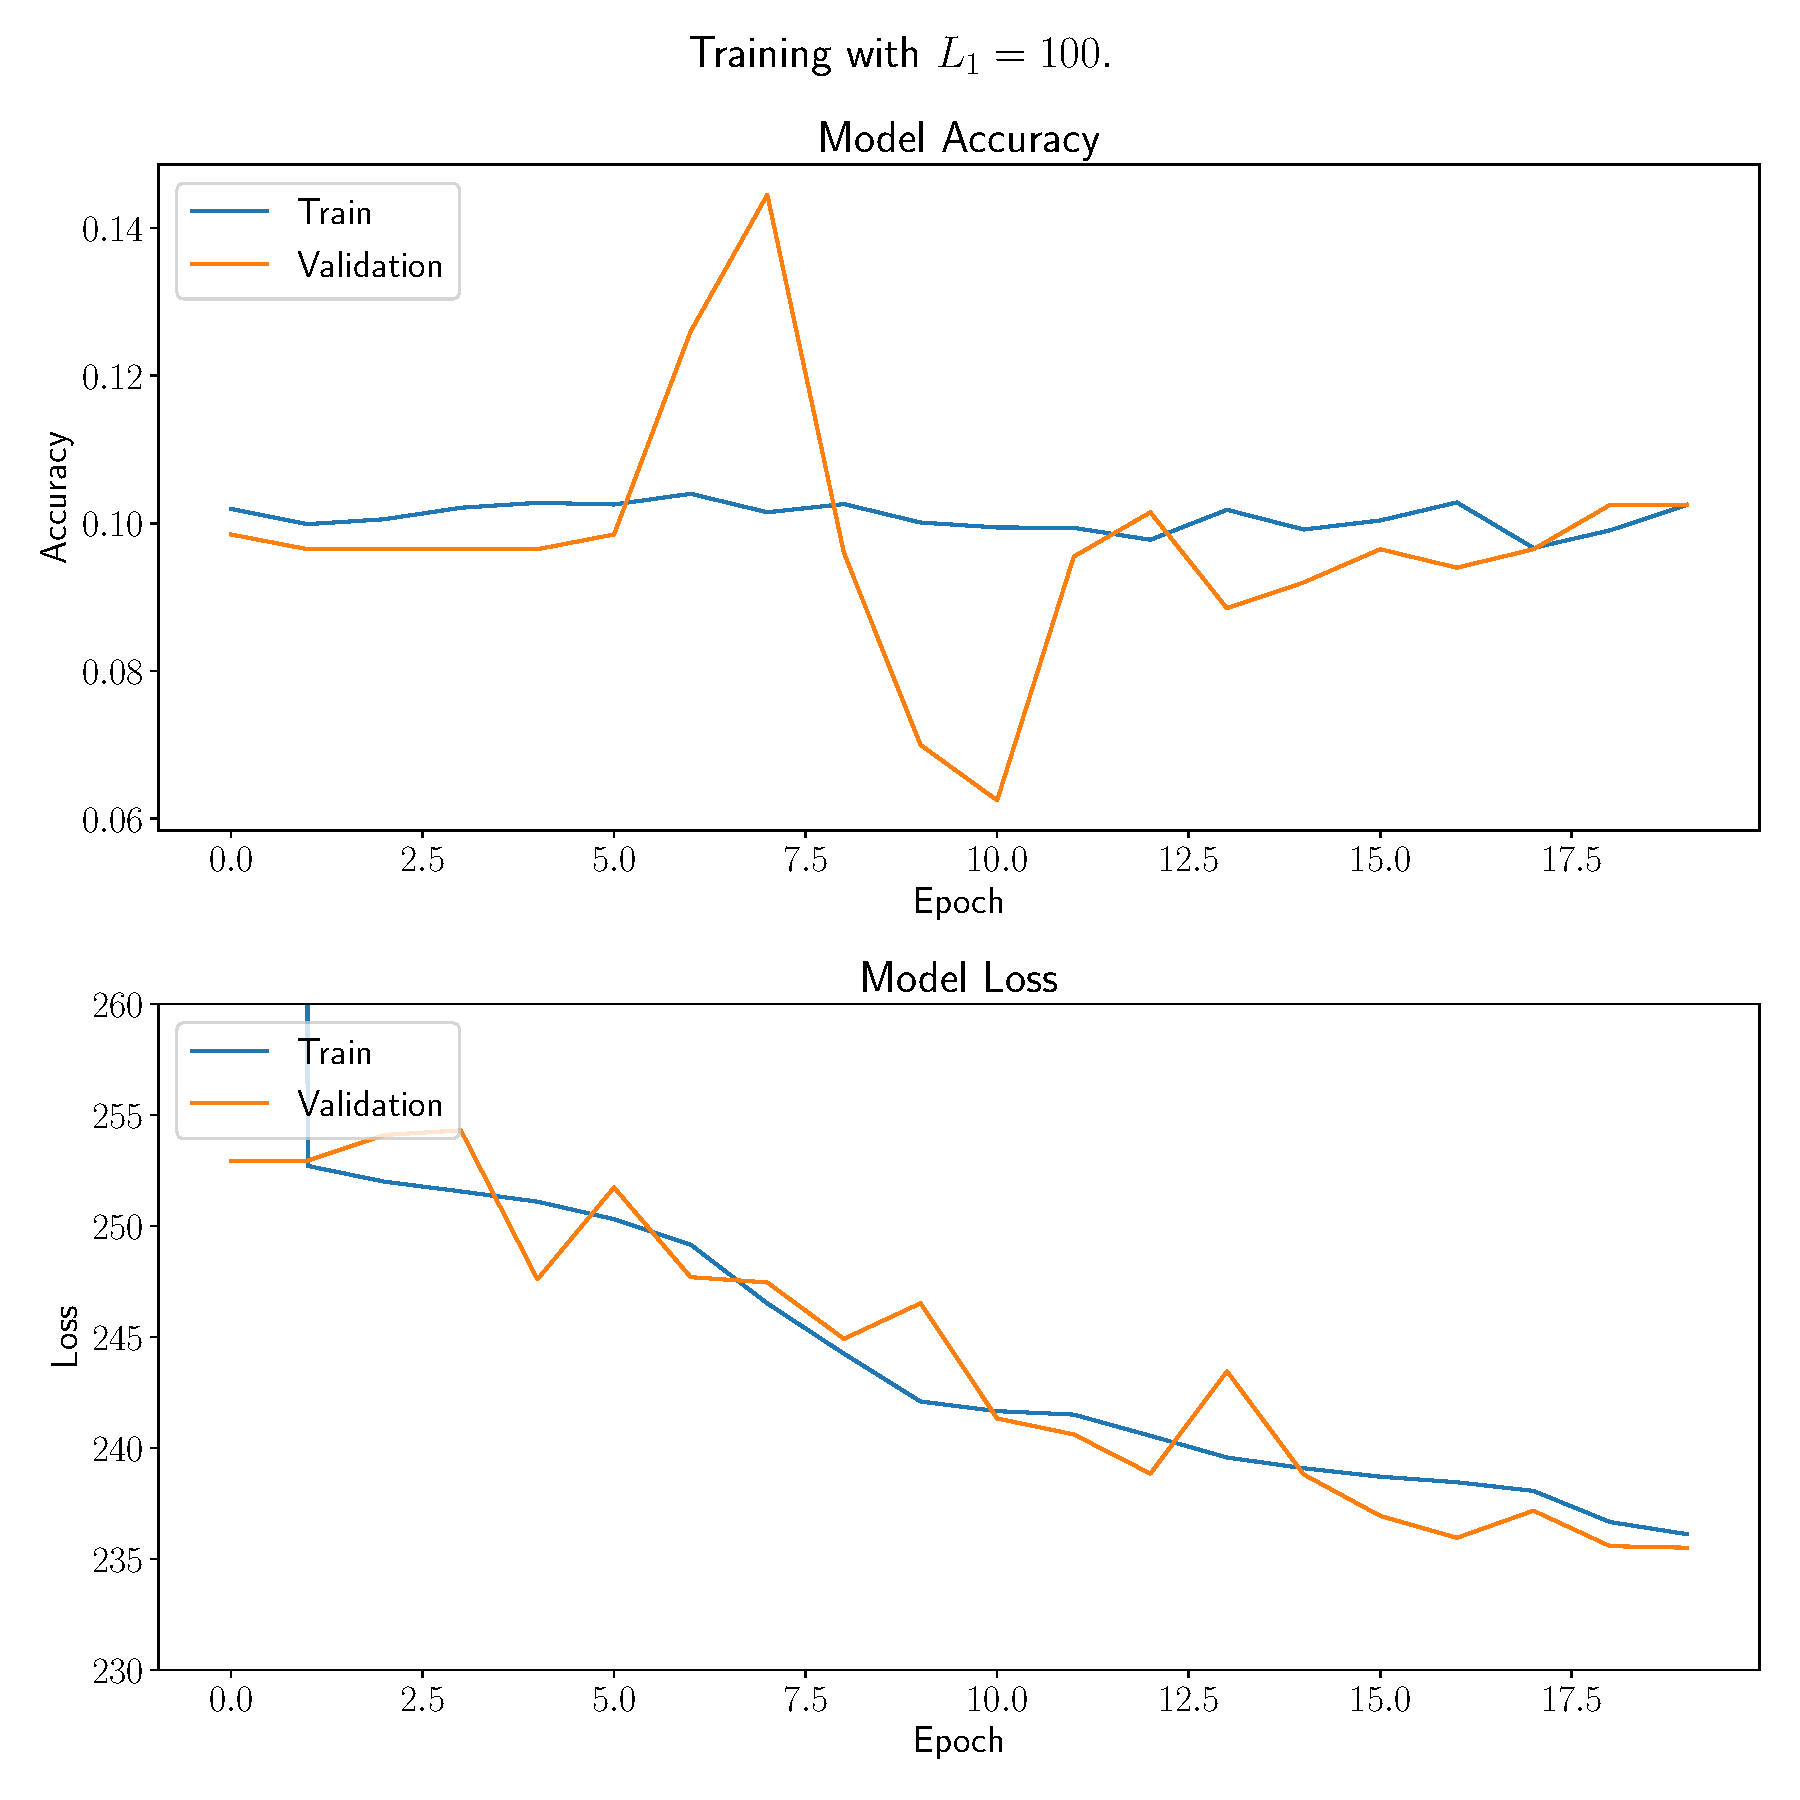
\includegraphics[width=0.49\textwidth]{exp/iibiv/100.acc-loss-lim.pdf}
    \par\end{centering}
    \caption{\label{fig:iibiv-acc-loss}A comparison of accuracy/loss on 
    training/test data from epochs 1 to 20 for different
    $L_1$ regularization terms, $0.0,0.00001,0.01,1000$.
    Each model is trained on 5K training samples.}
\end{figure}



\end{document}
